\documentclass{article}
\title{Simulate the trajectory of balloon}
\author{Haoen Huang, Liuyi Cui}
\date{20230426}
\usepackage{geometry}
\usepackage{url}
\geometry{a4paper,scale=0.8}
\usepackage{graphicx}
\usepackage{float}
\usepackage{indentfirst}
\usepackage[namelimits]{amsmath} %数学公式
\usepackage{amssymb}             %数学公式
\usepackage{color}
\usepackage{longtable}
\usepackage{listings}
\usepackage{multicol}%双栏
\usepackage{indentfirst}%缩进
\lstset{
language=Matlab,
numbers=left,
keywordstyle=\color{blue},
numberstyle=\tiny,
breaklines=true,
extendedchars=flase
}
\begin{document}
\maketitle

\begin{abstract}
In this study, we investigate the possibility of simulating the trajectory of a suspicious balloon traversing the United States using a random walk model with wind speed as the sole influencing factor. We present our findings by transforming the results of our random walk simulations into partial derivative functions, which enhances the clarity of our results. Based on our simulation data, we can reasonably assert that the balloon's trajectory can be partially replicated through a random walk simulation.
\end{abstract}
\setlength{\columnsep}{1cm}
\begin{multicols}{2}
\section{Introduction}
In February, news broke that a Chinese balloon had traversed the entire United States. According to the report, the balloon originated from Xinjiang, crossed the Pacific Ocean, entered Canada, and finally crossed the border into Montana. This news generated a lot of attention, with some labeling the balloon a Chinese spy balloon and alleging that it had a specific trajectory and purpose for entering the United States. However, the Chinese government denied these claims and stated that the balloon was a weather balloon, meaning its trajectory was random. We found this news intriguing and discovered some interesting mathematical connections. As such, our project aims to use various mathematical models to predict the balloon's trajectory under certain assumptions.





\section{Data discription}


\begin{figure*}[ht]
\begin{minipage}{0.45\linewidth}
\centering
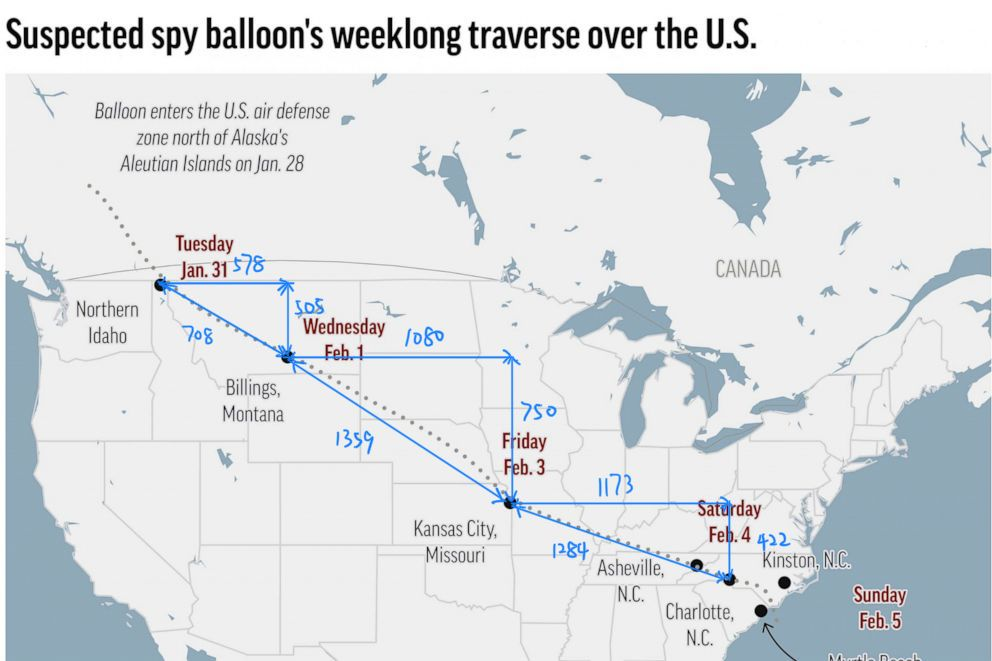
\includegraphics[width=0.6\linewidth]{graph/distance.png} 
\caption{Distance}
\label{distance}
\end{minipage}
\hfill
\begin{minipage}{0.45\linewidth}
\centering
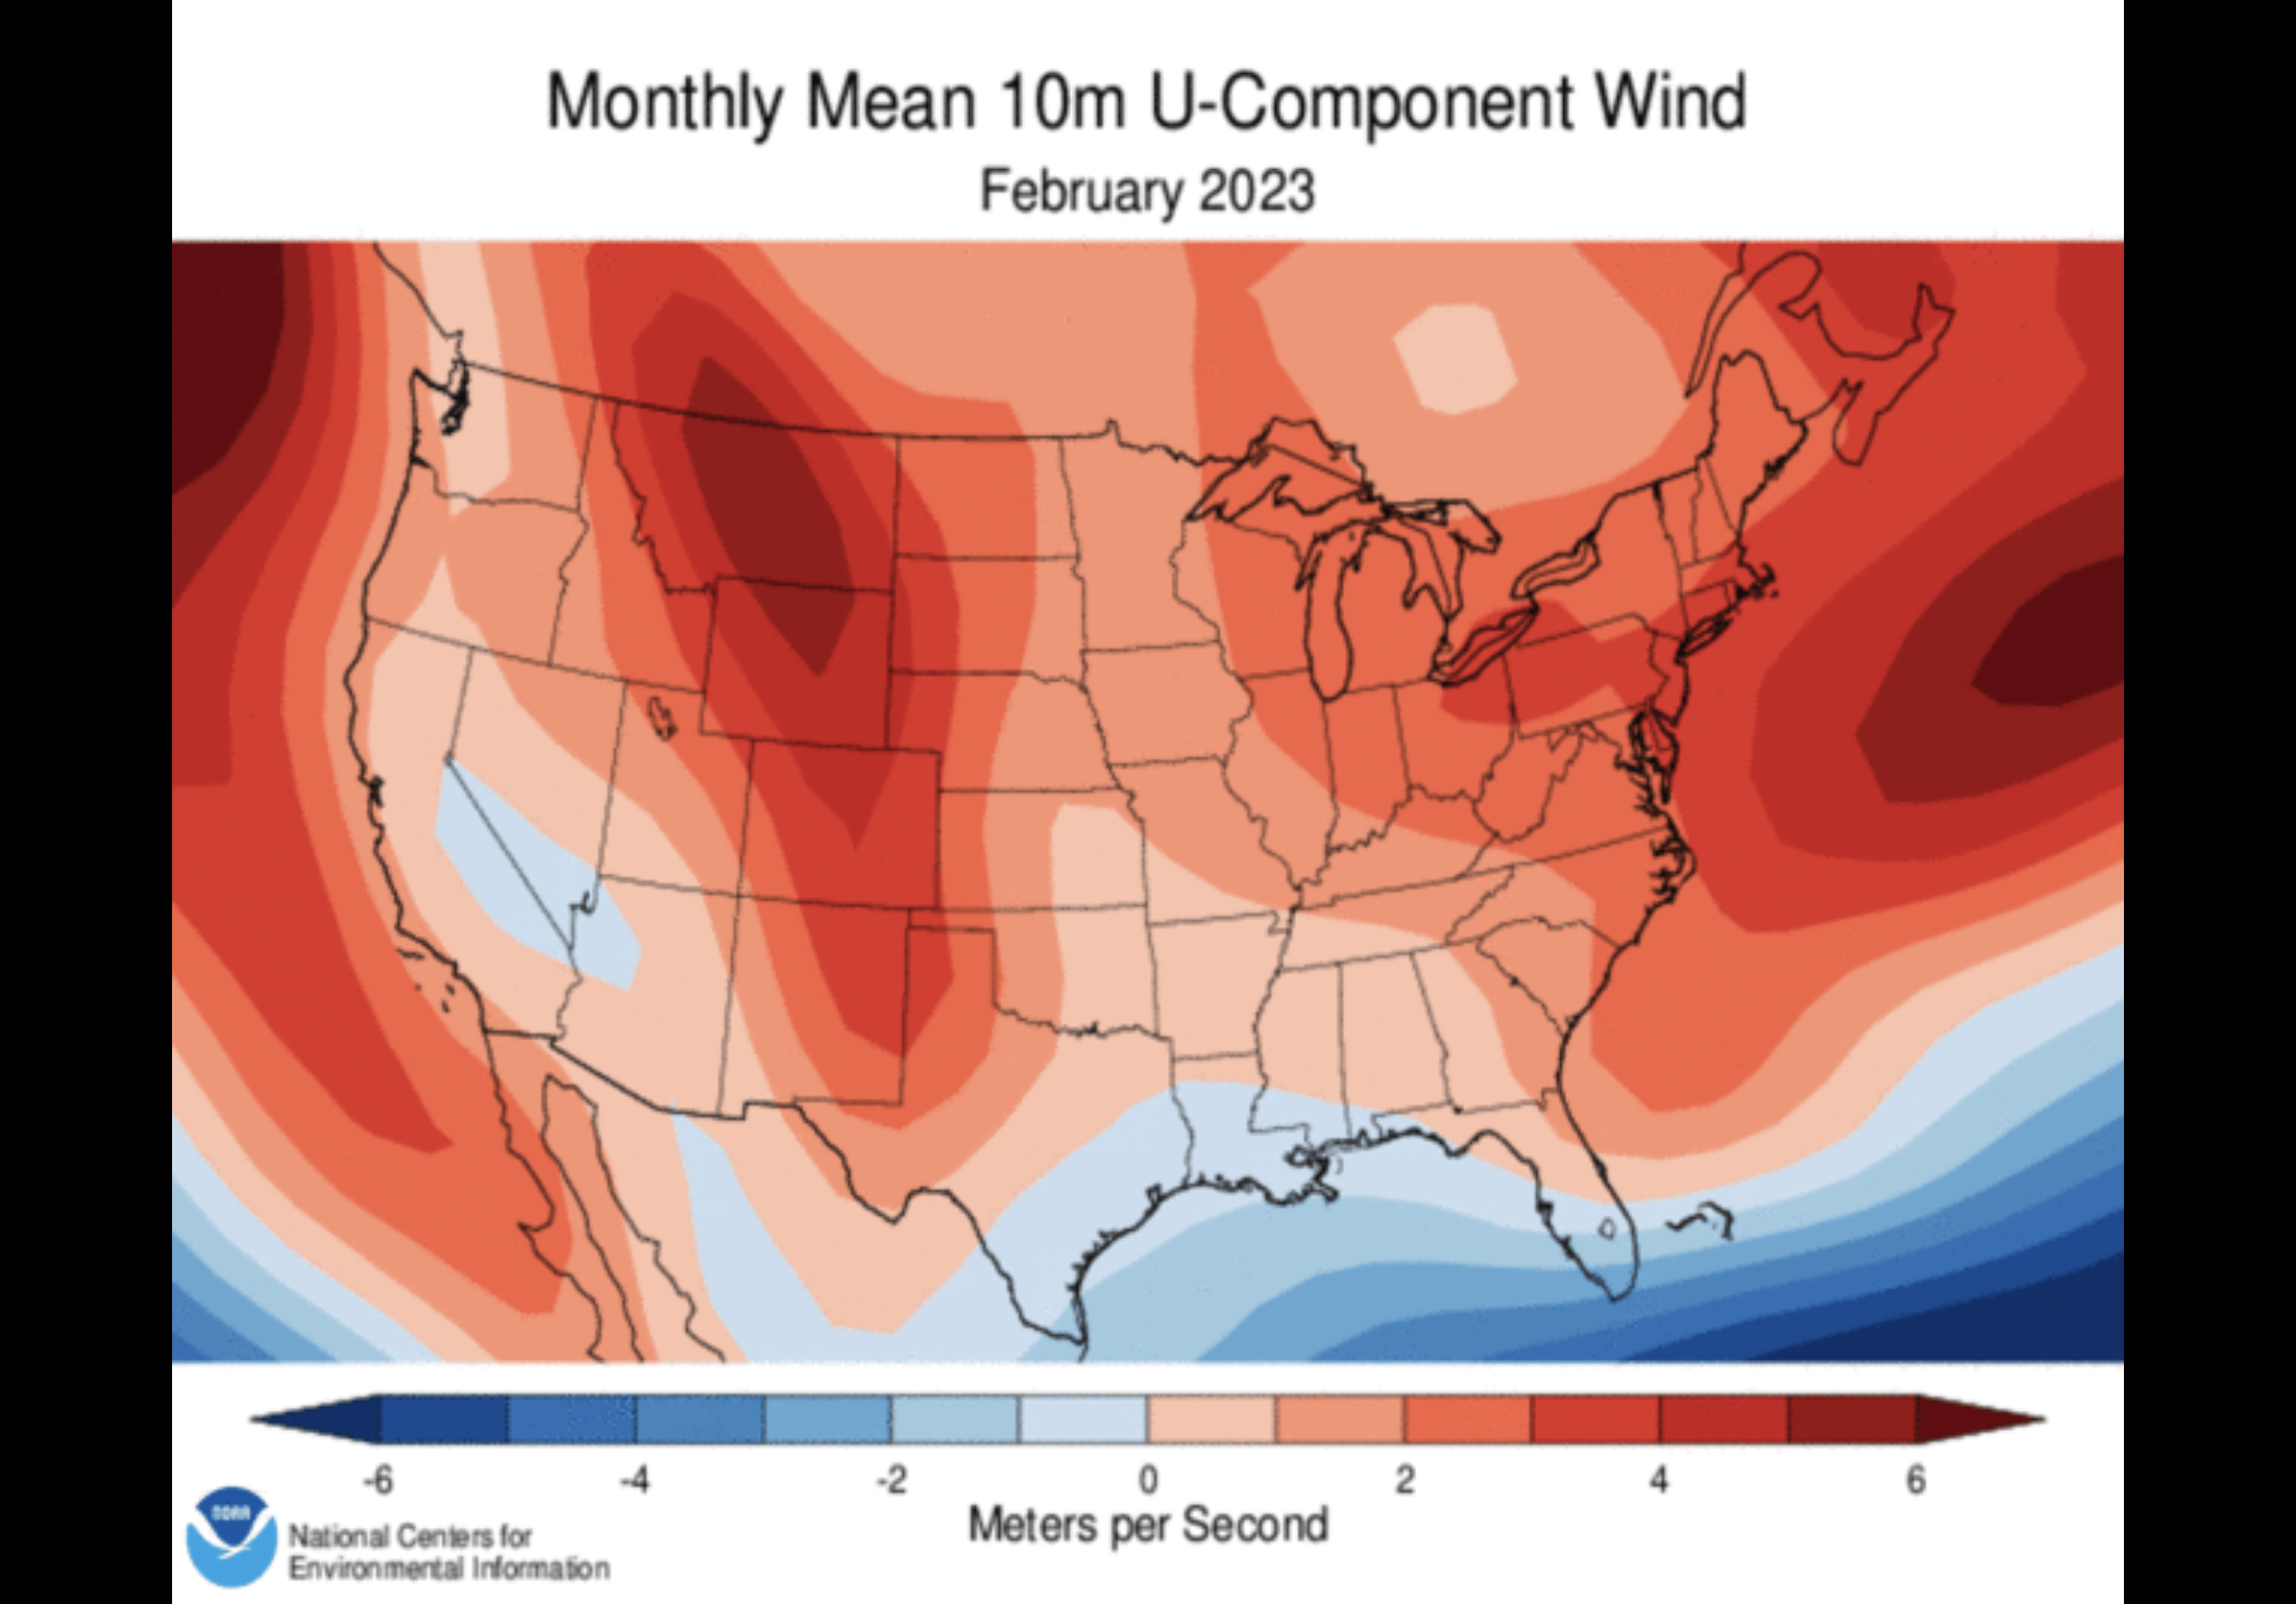
\includegraphics[width=0.6\linewidth]{graph/windspeed (1).png} 
\caption{Total wind speed}
\label{windspeed1}
\end{minipage}
\end{figure*}

\begin{figure*}[ht]
\begin{minipage}{0.45\linewidth}
\centering
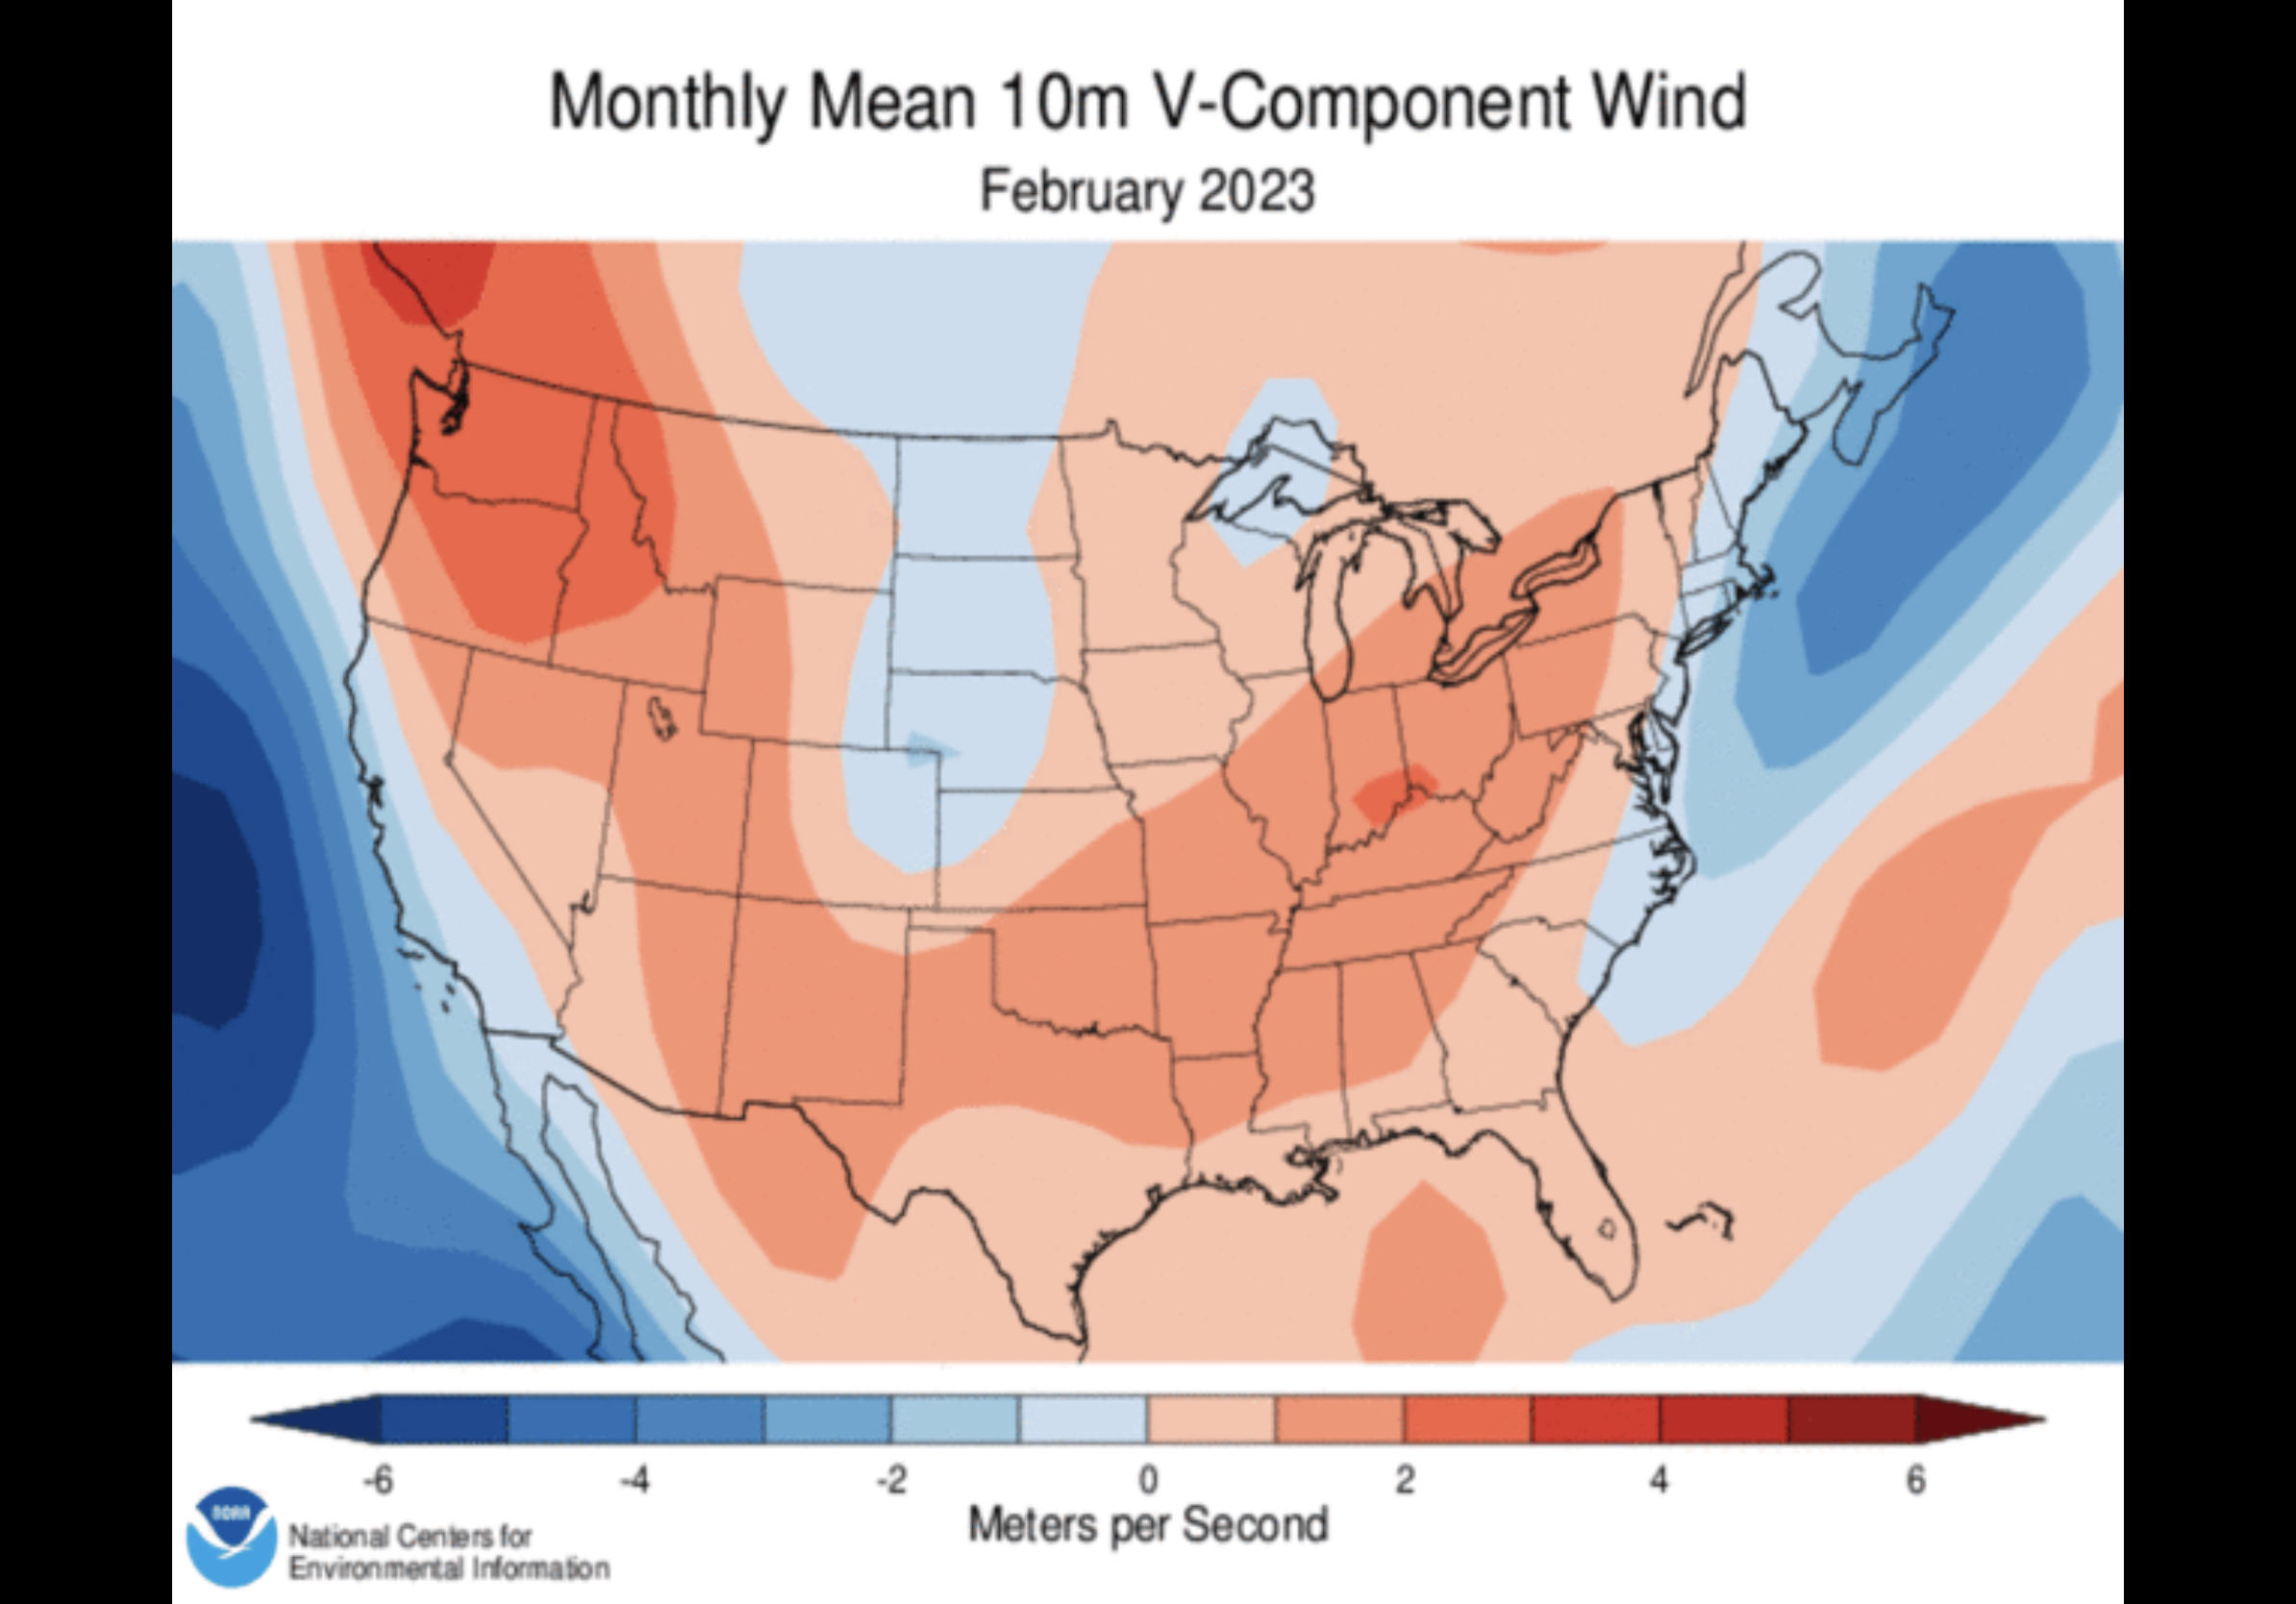
\includegraphics[width=0.6\linewidth]{graph/windspeed (2).png} 
\caption{Horizontal wind speed}
\label{windspeed2}
\end{minipage}
\hfill
\begin{minipage}{0.45\linewidth}
\centering
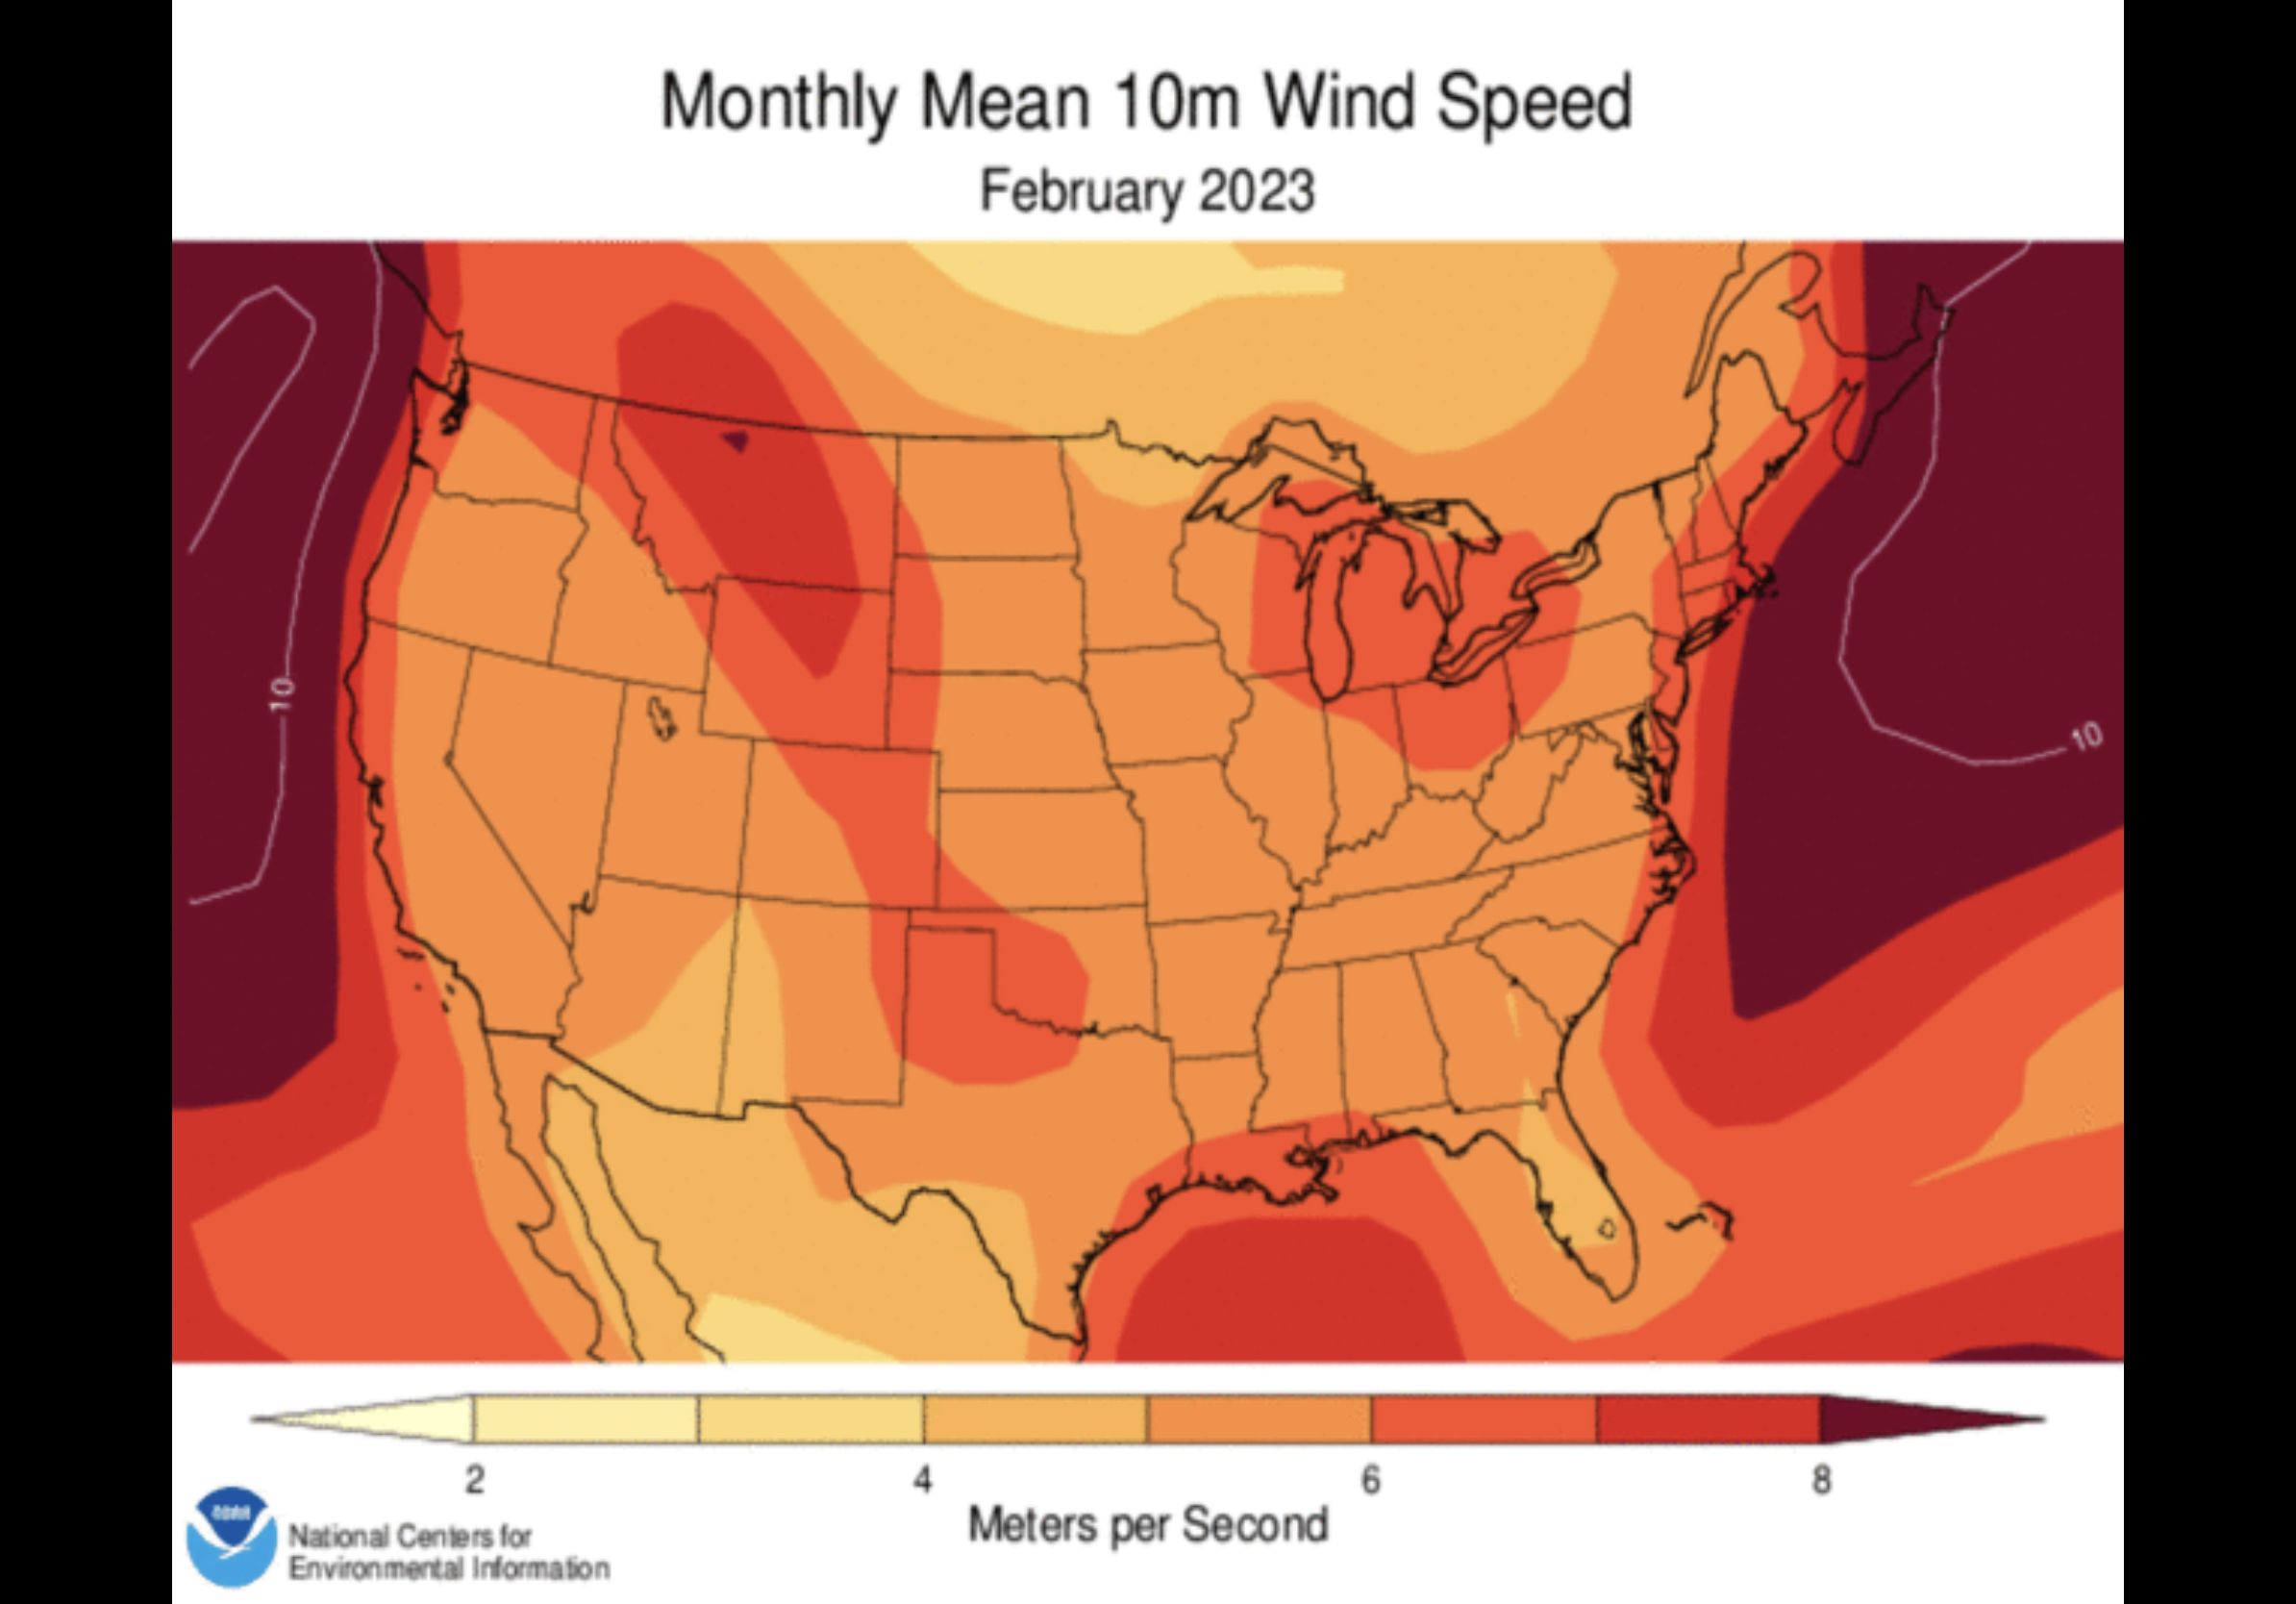
\includegraphics[width=0.6\linewidth]{graph/windspeed (3).png} 
\caption{Vertical wind speed}
\label{windspeed3}
\end{minipage}
\end{figure*}

\indent\setlength{\parindent}{2em}To establish our model, it is crucial to acquire the authentic trajectory of the balloon. We have obtained a graph \ref{distance}(from \cite{Tra_data}) illustrating the locations where the balloon was sighted. Subsequently, we diligently conducted a thorough investigation to determine the precise times when the balloon was observed. The initial sighting occurred in Northern Idaho at 20:00 on Tuesday, January 31st. Subsequently, the balloon moved to Billings at 20:00 on Wednesday, February 1st. On Friday, February 3rd, it was detected in Kansas City, and finally, on February 4th, it was sighted in Charlotte. These locations and corresponding time data are utilized as the balloon's positional information. We meticulously examined the distances between these locations and precisely annotated them on graph \ref{distance}. These meticulously acquired data will be employed in our one-dimensional and two-dimensional random walk simulations.\par
\indent\setlength{\parindent}{2em}We obtained the average wind speed heatmap for the month of February from the official website of the United States climate government\cite{Wind_data}. This dataset encompasses horizontal windspeed (figure \ref{windspeed2}), vertical windspeed (figure \ref{windspeed3}), and total windspeed (figure \ref{windspeed1}). Subsequently, we extracted the wind speed data corresponding to the trajectory of the balloon.



\section{Hypothesis and Data analysis}
In our proposed model, we make the assumption that the trajectory of the balloon is solely determined by wind patterns, treating it as an erratic aircraft that has unintentionally entered the United States. Based on this hypothesis, we further assume that the average wind direction aligns with the direction of the balloon's trajectory.\par
\indent\setlength{\parindent}{2em}Using the aforementioned positional and wind data, we are able to compute the average speed of the balloon. We segment the trajectory into three distinct sections and compare the balloon's speed to the corresponding wind speed. During the initial two sections, we observe a remarkable similarity between the two. However, in the third section, the balloon's speed undergoes a substantial enhancement. This deviation from the average wind speed is significant enough for us to conclude that this particular section should be excluded from further analysis.



\section{One dimension randomwalk simulation}
\subsection{Model building}
To simulate the trajectory, we employ a one-dimensional biased random walk instead of an unbiased random walk. This choice allows us to incorporate the influence of wind speed. Equation (\ref{eq1}) is utilized to establish the relationship between wind speed and the random walk. It is assumed that the intended destination of the balloon is towards the right side. In this equation, $q$ represents the probability of the balloon moving to the right during a single step of the random walk. $\Delta x$ and $\Delta t$ denote the distance and time covered by a single random walk step respectively. 
\begin{equation}
(2q-1)\frac{\Delta x}{\Delta t}= Expected speed = Wind speed
\label{eq1}
\end{equation}
\indent\setlength{\parindent}{2em}There are three parameters in equation (\ref{eq1}). To ensure the accuracy of our model, we fix the values of $\Delta x$ and $\Delta t$ as $\Delta x = 5$ km and $\Delta t = \frac{1}{10}$ h = 6 min. Subsequently, we utilize the wind speed data to calculate the value of $q$. In the first section, we obtain $q_1 = 0.68$, while in the second section, we find $q_2 = 0.71$. These calculated values of $q$ enable us to conduct random walk simulations using the specified parameters.\par

\indent\setlength{\parindent}{2em}To facilitate a clearer understanding of the random walk results, we establish a connection between the random walk and the heat diffusion equation. We define $P(x,N)$ as the probability of the balloon being located at position $x$ at time $N\Delta t$. The position of the balloon at time $(N+1)\Delta t$ is determined by its position at time $N\Delta t$. The relationship between these positions is described by equation (\ref{eq2}).
\begin{equation}
P(x,N+1)=\sum_y \pi(x,y)P(y,N)
\label{eq2}
\end{equation}
\indent\setlength{\parindent}{2em}We apply Taylor series to equation(\ref{eq2}), and we get the partial dirivative equation(\ref{eq3}). 
\begin{equation}
\frac{\partial P_x}{\partial t}=(1-2q)\frac{\Delta x}{\Delta t}+\frac{1}{2}\frac{\Delta x^2}{\Delta t}\frac{{\partial}^2 P_x}{\partial x^2}
\label{eq3}
\end{equation}
\subsection{Methods}
To solve the partial derivative equation (\ref{eq3}), we employ two methods: the Pdebe method in Matlab and a numerical solution approach. In the numerical solution, we represent the probability of the balloon's position at $i\Delta x$ and time $n\Delta t$ as $P_{i}^{n}$. Applying the FTCS (Forward-Time Central-Space) method to equation (\ref{eq3}), we obtain equation (\ref{eq4}).
\begin{equation}
\begin{split}
P^{(n+1)}_{i+1}=&P^{(n)}_i+(1-2q)\frac{(P^{(n)}_{i+1}-P^{(n)}_{i-1})}{2}\\
&+\frac{(P^{(n)}_{i+1}-2P^{(n)}_{i}+P^{(n)}_{i-1})}{2}
\label{eq4}
\end{split}
\end{equation}
\indent\setlength{\parindent}{2em}Equation (\ref{eq4}) represents the recursion formula that allows us to calculate $P_{i}^{N}$, which represents the probability of the balloon's position at the end time of each trajectory section.

It is important to note that both methods employed in this study are numerical methods. Furthermore, it is worth mentioning that we are primarily interested in the relative proportions of the probabilities rather than their absolute values. Therefore, after performing the necessary calculations, we rescale the results to ensure that the sum of the probabilities equals 1.

\subsection{Result}
\begin{figure*}[ht]
\begin{minipage}{0.45\linewidth}
\centering
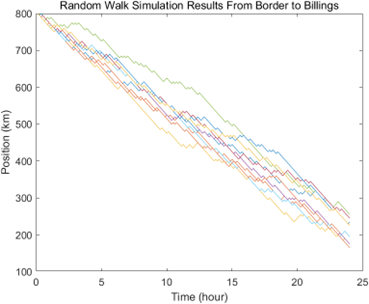
\includegraphics[width=0.8\linewidth]{graph/1ds1.png} 
\caption{1-D random walk simulation section 1}
\label{1ds1}
\end{minipage}
\hfill
\begin{minipage}{0.45\linewidth}
\centering
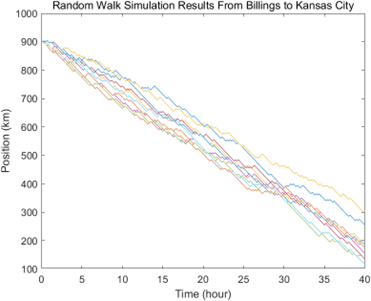
\includegraphics[width=0.8\linewidth]{graph/1ds2.png} 
\caption{1-D random walk simulation section 2}
\label{1ds2}
\end{minipage}
\end{figure*}
\begin{figure*}[ht]
\begin{minipage}{0.45\linewidth}
\centering
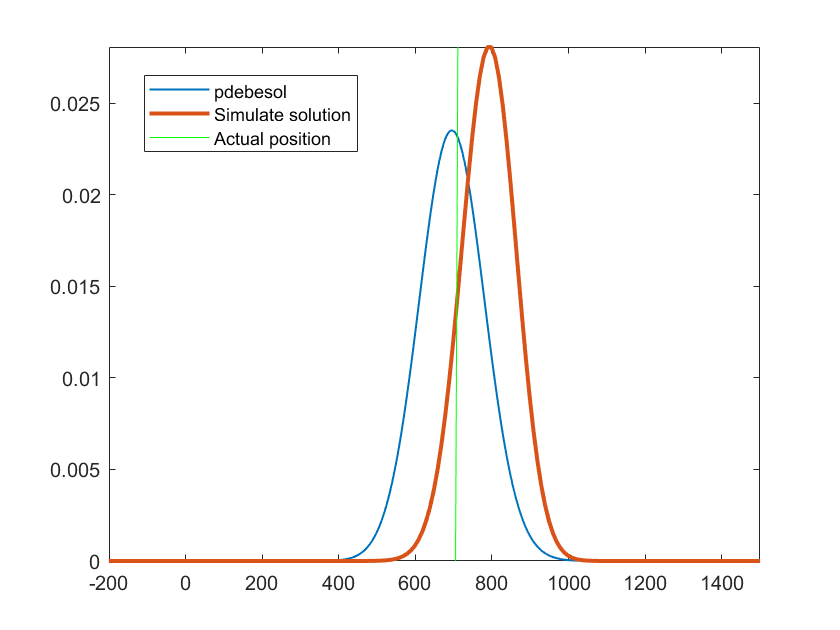
\includegraphics[width=0.8\linewidth]{graph/1ddis1.png} 
\caption{1-D Probability simulation section 1}
\label{1dps1}
\end{minipage}
\hfill
\begin{minipage}{0.45\linewidth}
\centering
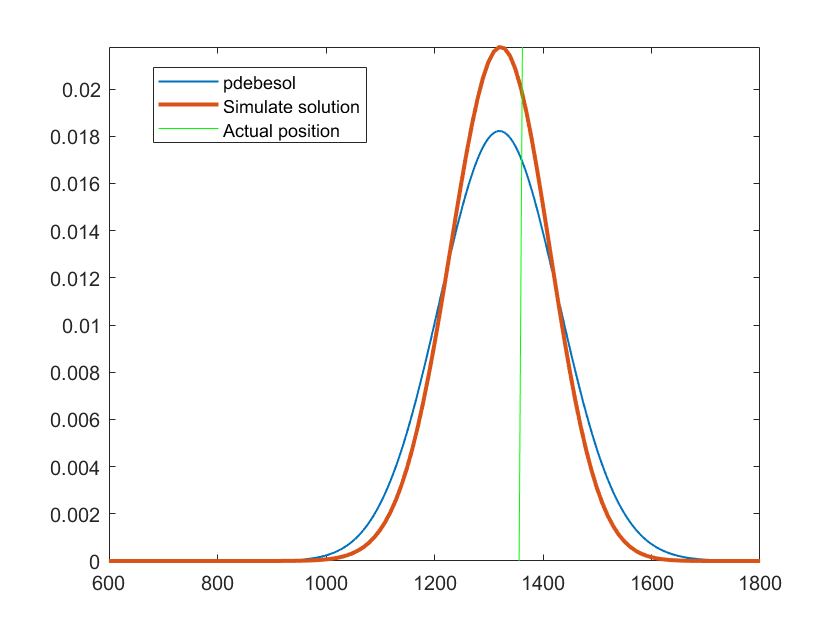
\includegraphics[width=0.8\linewidth]{graph/1ddis2.png} 
\caption{1-D Probability simulation section 2}
\label{1dps2}
\end{minipage}
\end{figure*}
Figure (\ref{1ds1}) and Figure (\ref{1ds2}) depict the outcomes of 10 random walk simulations for trajectory section 1 and section 2, respectively. Each simulation is represented by a different color. On the other hand, Figure (\ref{1dps1}) and Figure (\ref{1dps2}) display the probabilities at the end time of trajectory section 1 and section 2, respectively. The green line in these figures represents the actual position of the balloon.






\section{Two dimension randomwalk simulation}
\subsection{Model building}
After completing the simulation of the one-dimensional random walk, we proceed to the two-dimensional component. Instead of directly simulating a two-dimensional random walk, we construct two separate one-dimensional random walks for the horizontal and vertical directions. We continue to utilize equation (\ref{eq1}) to establish the random walk in both directions. However, this time we incorporate the wind speed data obtained from Figure (\ref{windspeed2}) for the horizontal direction and Figure (\ref{windspeed3}) for the vertical direction. Similarly, we maintain a fixed $\Delta x$ value of $5$ km and $\Delta t$ value of $0.1$ h.

For the horizontal direction, we calculate the values of $q_{1h} = 0.68$ and $q_{2h} = 0.72$ in each section. On the other hand, for the vertical direction, we obtain $q_{1v} = 0.68$ and $q_{2v} = 0.66$ in each respective section. Subsequently, we apply the Taylor series expansion to the relation function (\ref{eq2}) and derive the corresponding partial derivative equation (\ref{eq3}) for each direction.







\subsection{Methods}
In the current scenario, we solely rely on numerical methods to solve the two-dimensional partial derivative equation (\ref{eq3}). Due to its two-dimensional nature, we calculate the probabilities separately for each dimension, denoted as $P_h$ for the horizontal direction and $P_v$ for the vertical direction.

To construct the two-dimensional probability matrix, we combine these individual probabilities using equation (\ref{eq5}). This equation allows us to establish the joint probability distribution, taking into account both the horizontal and vertical dimensions.
\begin{equation}
P=P_v^{T}\times P_h
\label{eq5}
\end{equation}



\subsection{Result}
\begin{figure*}[ht]
\begin{minipage}{0.45\linewidth}
\centering
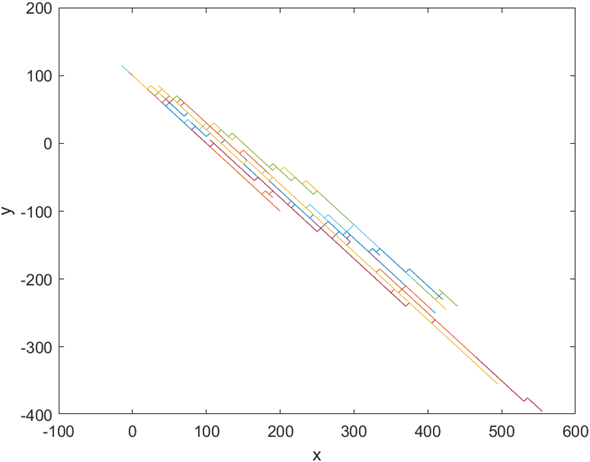
\includegraphics[width=0.8\linewidth]{graph/2ds1.png} 
\caption{2-D random walk simulation section 1}
\label{2ds1}
\end{minipage}
\hfill
\begin{minipage}{0.45\linewidth}
\centering
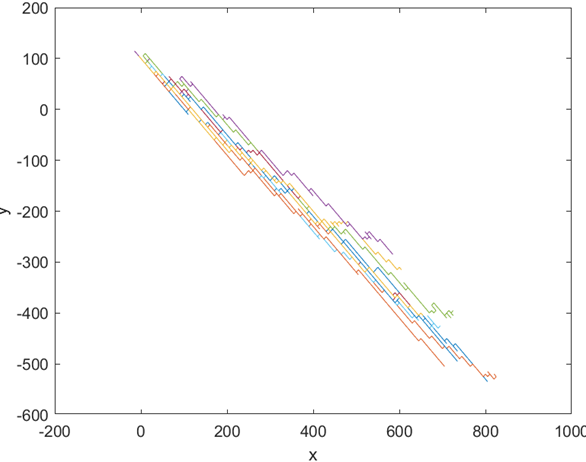
\includegraphics[width=0.8\linewidth]{graph/2ds2.png} 
\caption{2-D random walk simulation section 2}
\label{2ds2}
\end{minipage}
\end{figure*}
\begin{figure*}[ht]
\begin{minipage}{0.45\linewidth}
\centering
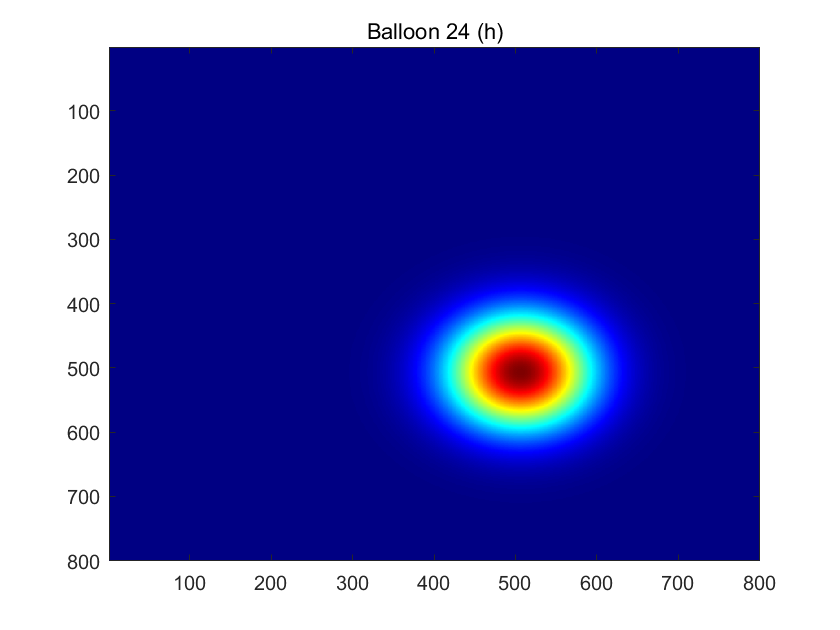
\includegraphics[width=0.8\linewidth]{graph/2ddis1.png} 
\caption{2-D Probability simulation section 2}
\label{2dps1}
\end{minipage}
\hfill
\begin{minipage}{0.45\linewidth}
\centering
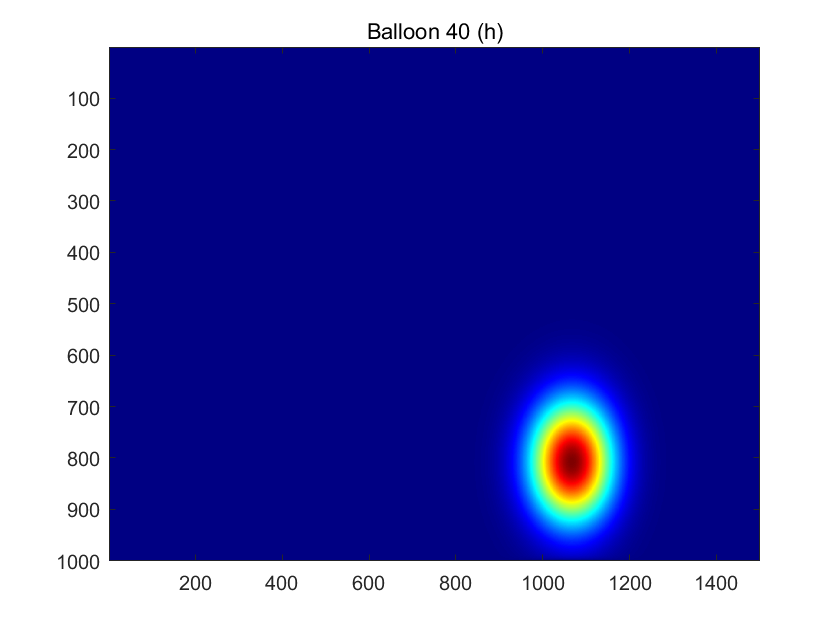
\includegraphics[width=0.8\linewidth]{graph/2ddis2.png} 
\caption{2-D Probability simulation section 2}
\label{2dps2}
\end{minipage}
\end{figure*}
\indent\setlength{\parindent}{2em}Figure (\ref{2ds1}) and Figure (\ref{2ds2}) present the simulation results of the 10 instances of the two-dimensional random walk. Each simulation is displayed in a separate color, allowing for visual comparison.

In Figure (\ref{2dps1}) and Figure (\ref{2dps2}), we observe heatmaps representing the final positions of the simulations. The heatmaps utilize a color gradient, where a redder color indicates a higher probability of the final position being located in that region. These heatmaps offer a visual representation of the likelihood distribution of the balloon's final position after the random walk simulations.





\section{Conclusions}
In our random walk simulations, we observe that a majority of the results converge to the actual positions. By examining the probability simulations shown in Figure (\ref{1dps1}) and Figure (\ref{1dps2}), we can conclude that the simulations closely align with the final positions. Although there may be variations in the actual wind speed on the specific day compared to the average wind speed we used in our simulations, the overall success of our simulation supports the claim that the balloon's trajectory can be effectively simulated by a random walk model.

However, it is important to acknowledge the limitations and inadequacies of our research. Firstly, the wind data we used was limited to the upper air, necessitating the utilization of ground-level wind speed for our simulations. This may introduce some inaccuracies in our results. Additionally, we were unable to find an analytical solution for the partial derivative equation (\ref{eq3}), and therefore relied solely on numerical methods. Furthermore, our simulation only accounted for the first two trajectory sections where the balloon's speed closely matched the wind speed. We were unable to determine the reason behind the significant increase in speed observed in the third section. Addressing these limitations and challenges may require more in-depth research and analysis, potentially involving advanced machine learning techniques.
\end{multicols}
\nocite{*}
\bibliographystyle{plain}
\bibliography{Reference}








\end{document}